%%%
%
% $Autor: Wings $
% $Datum: 2021-05-14 $
% $Pfad: GitLab/MLEdgeComputer $
% $Dateiname: CAMov2640 
% $Version: 4620 $
%
% !TeX spellcheck = de_GB
%
%%%

\chapter{Kamera-Modul ArduCAM OV2640}

\section{OV7675 Camera Module}

\begin{itemize}
  \item 0.3 MP CMOS image sensor
  \item active array size: 640×480
  \item output formats: YUV422, Raw RGB, ITU656, RGB565
  \item  input clock frequency: 1.5 $\approx$ 27 MHz
  \item maximum image transfer rate: VGA 30fps, QVGA 60fps, QQVGA 240pfs
  \item pixel size: 2.5 $\mu m \times 2.5 \mu m$
  \item image area: 1640  $\mu m \times 1220  \mu m$
\end{itemize}



\begin{itemize}
    \item  \URL{https://www.arducam.com/products/camera-breakout-board/0-3mp-ov7675/}
    \item  \URL{https://github.com/ArduCAM/ArduCAM_USB_Camera_Shield}
    \item  \URL{https://github.com/ArduCAM/Arduino}
\end{itemize}



\begin{figure}
    \begin{center}
        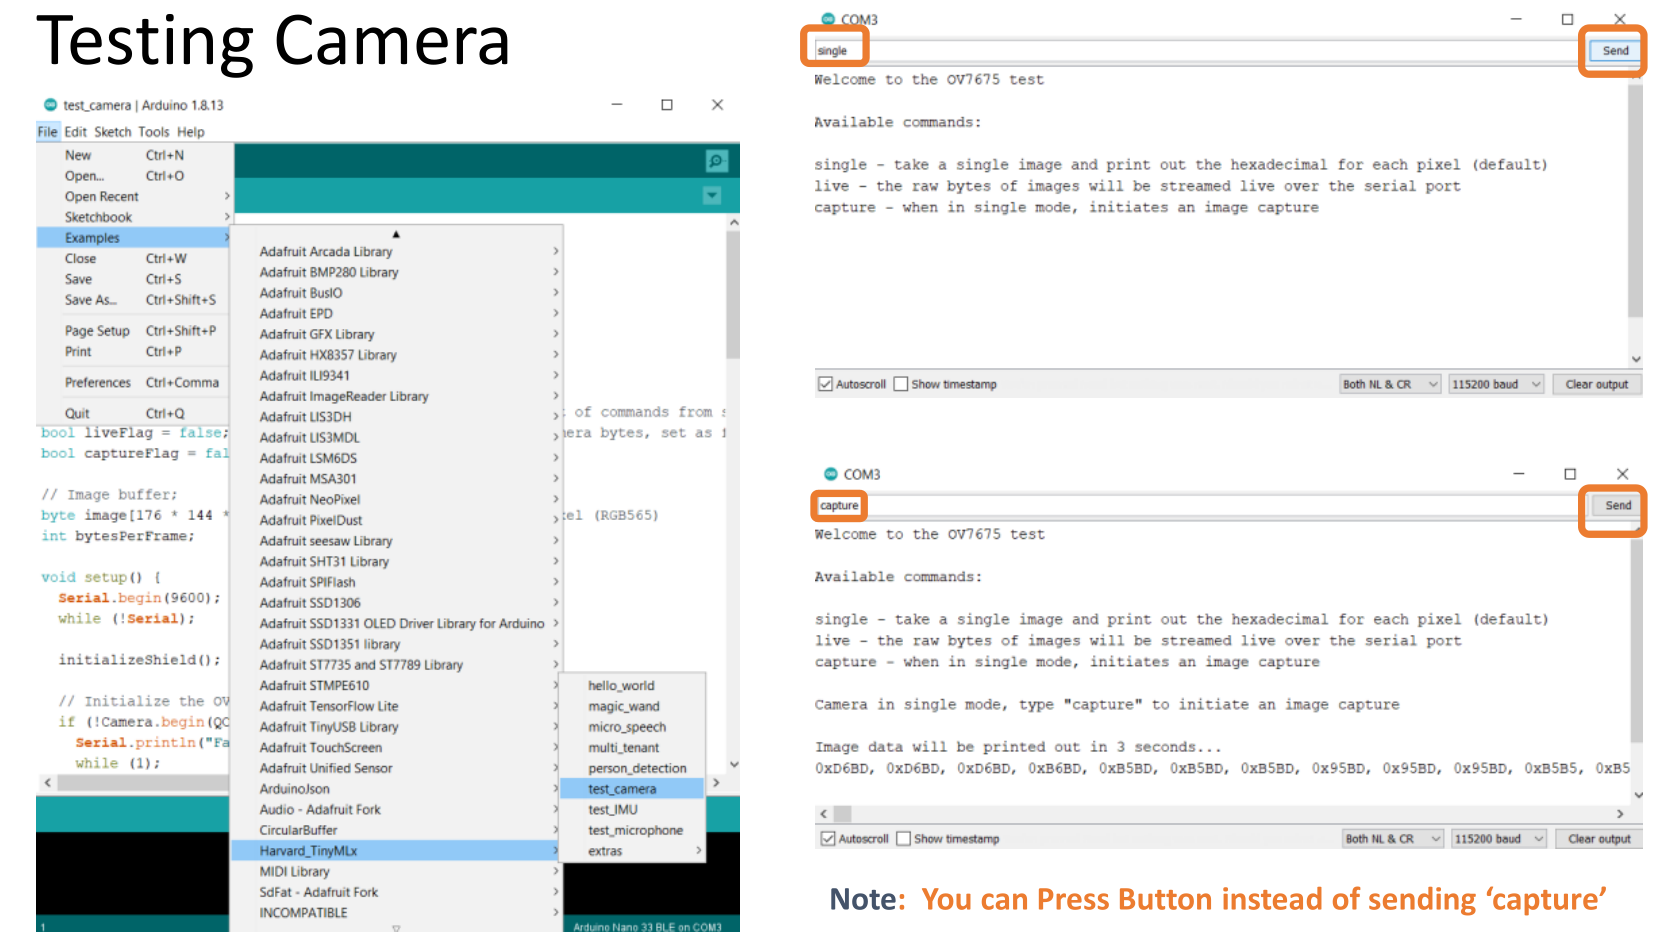
\includegraphics[scale=0.13]{CAM/ov2640/TestCam}
        
        \caption{Test program}
    \end{center}    
\end{figure}

\begin{figure}
    \begin{center}
        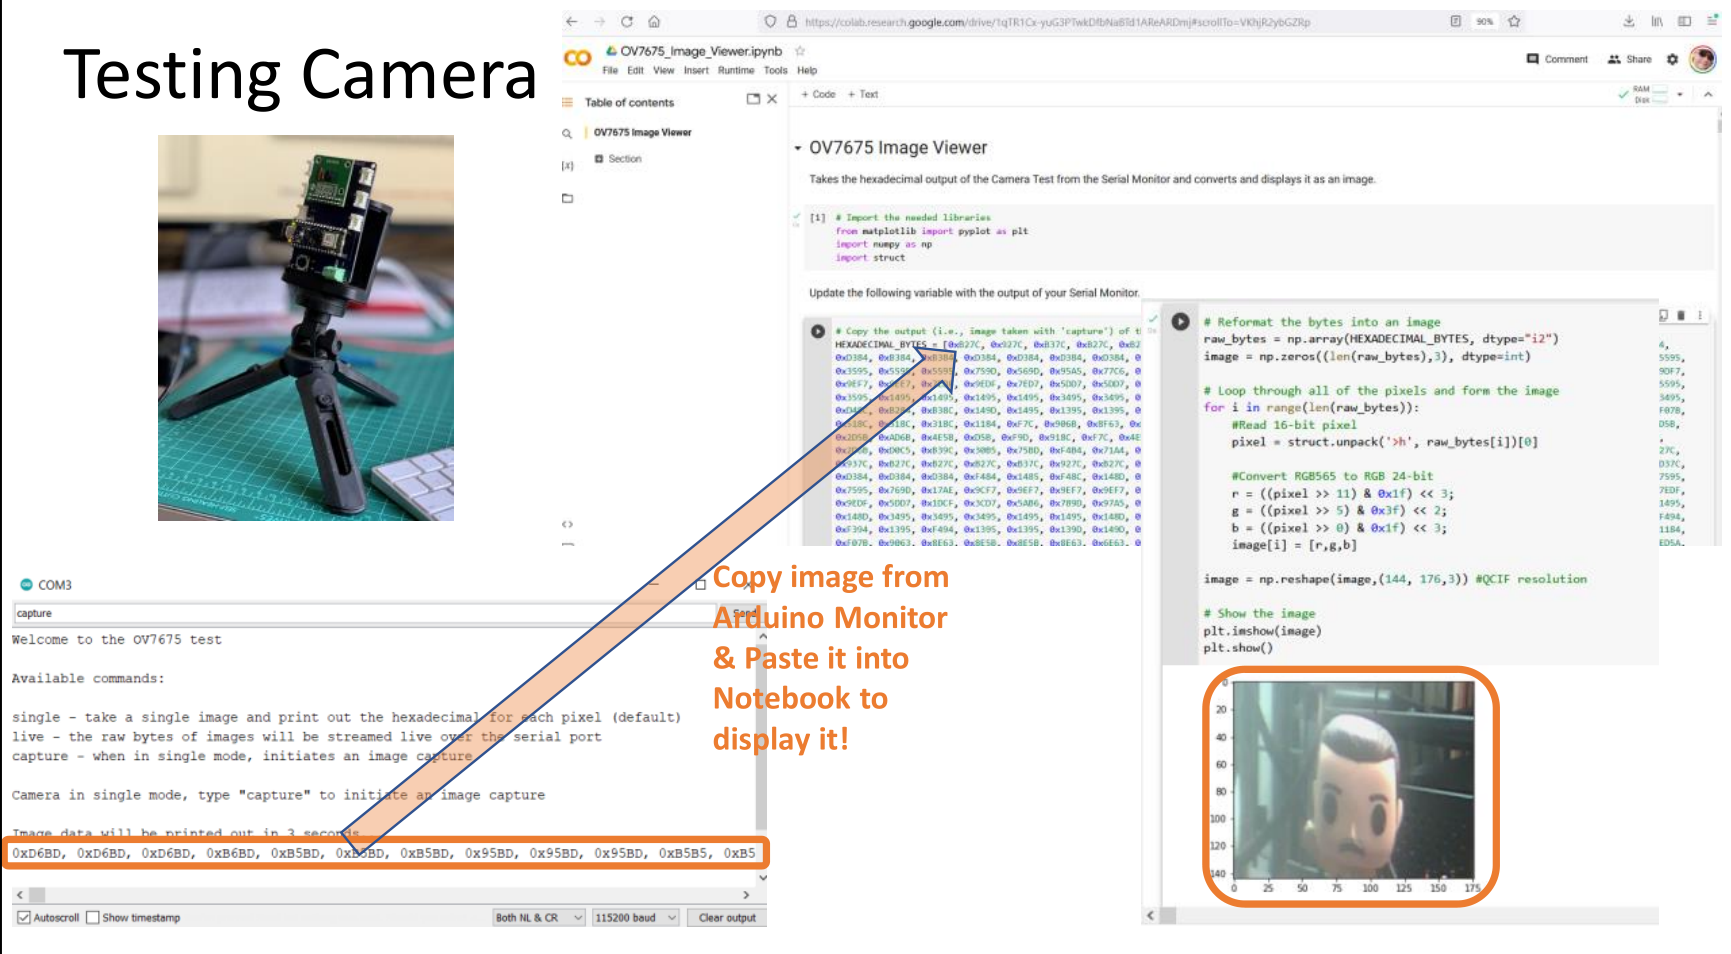
\includegraphics[scale=0.13]{CAM/ov2640/TestCam02}
        
        \caption{Test program}
    \end{center}    
\end{figure}


\section{Indroduction}

ArduCAM is Arduino based open source camera platform which is well mated to Arduino boards. It is a high definition 2MP SPI camera, which reduce the complexity of the camera control interface. It integrates 2MP CMOS image sensor OV2640, and provides miniature size, as well as the easy to use hardware interface and open source code library. The ArduCAM mini can be used in any platforms like Arduino, Raspberry Pi, Maple, Chipkit, Beaglebone black, as long as they have SPI and I2C interface and can be well mated with standard Arduino boards. The figure ~\ref{Arducam} shows the mini ArduCAM Camera. The mini ArduCAM OV2640 is well suited for tinyML application, it is easy to configure with Arduino boards. For making the ML applications, especially Images caputuring, object and gesture detection, it supports to take capture and send back to Arduino microcontroller for getting desire results. \href{https://www.arducam.com/product/arducam-2mp-spi-camera-b0067-arduino/}{[Arducam]}



\url{https://www.arducam.com/ov2640/}

\url{https://www.arducam.com/focal-length-calculator/}

\section{Produktbeschreibung}

Arducam-M-2MP ist eine optimierte Version von Arducam Shield Rev.C und ist eine hochauflösende 2MP-SPI-Kamera, die die Komplexität der Kamerasteuerung verringert. Sie verfügt über einen 2-MP-CMOS-Bildsensor OV2640 und hat eine Miniaturgröße sowie eine einfach zu bedienende Hardware-Schnittstelle und die Open-Source-Code-Bibliothek. Die Arducam Mini-Kamera kann auf allen Plattformen wie Arduino, Raspberry Pi, Maple, Chipkit, Beaglebone Black verwendet werden, solange sie über eine SPI- und I2C-Schnittstelle verfügen und mit Standard-Arduino Boards verbunden werden können. Die Arducam Mini-Kamera bietet nicht nur die Möglichkeit, eine Kamera-Schnittstelle hinzuzufügen, die in einigen Mikrocontrollern nicht vorhanden ist, sondern bietet auch die Möglichkeit, mehrere Kameras zu einem einzigen Mikrocontroller hinzuzufügen.

\bigskip

Anwendung:
\begin{itemize}
  \item IoT-Kameras.
  \item Roboterkameras.
  \item Wildlife-Kameras.
\end{itemize}

Andere batteriebetriebene Produkte.
Kann auf Plattformen wie MCU, Raspberry Pi, ARM, DSP, FPGA verwendet werden.

\bigskip

Eigenschaften:

\begin{itemize}
  \item 2-Megapixel-Bildsensor OV2640.
  \item M12-Mount- oder CS-Mount-Objektivhalter mit wechselbaren Objektivoptionen.
  \item IR-empfindlich mit entsprechender Objektivkombination.
  \item I2C-Schnittstelle für die Sensorkonfiguration.
  \item SPI-Schnittstelle für Kamera-Befehle und Datenstrom.
  \item Alle E/A-Anschlüsse sind für 5 V/3,3 V geeignet.
  \item Unterstützt JPEG-Komprimierungsmodus, Einzel- und Mehrfachaufnahmemodus, einmaliges Erfassen mehrerer Lesevorgänge, Burst-Lese-Operation, Niedrige-Energie-Modus usw..
  \item Kann mit Standard-Arduino-Boards verbunden werden.
  \item Open-Source-Code-Bibliothek für Arduino, STM32, Chipkit, Raspberry Pi, BeagleBone Black.
  \item Schlanke Form.
\end{itemize}

\bigskip

Lieferumfang:

1 x Arducam Mini-Modul Kameraschutz mit OV2640 2 MP, Objektiv, für Arduino UNO Mega2560 Board.

Hinweis: Arduino UNO ist nicht enthalten.

\bigskip


\url{https://www.amazon.com/dp/B07D58GDDV/ref=sr_1_17_sspa?__mk_de_DE=ÅMÅŽÕÑ&dchild=1&keywords=arducam&qid=1622358684&sr=8-17-spons&psc=1&spLa=ZW5jcnlwdGVkUXVhbGlmaWVyPUEyWUdNSVhJSFNUQUtLJmVuY3J5cHRlZElkPUEwNjI4NTQxM0RNQ0I2NDJDNzdUTCZlbmNyeXB0ZWRBZElkPUEwMjEyMjUwNTFSVjM2SzZFM1VCJndpZGdldE5hbWU9c3BfYXRmX25leHQmYWN0aW9uPWNsaWNrUmVkaXJlY3QmZG9Ob3RMb2dDbGljaz10cnVl0}

    
Raspberry Pi Kamerakabel, iUniker 15-poliges Flachbandkabel, Pi Kamera Flex Kabel, Flex CSI Kabel 50 cm/1 m/2 m für Raspberry Pi 3B+, 3B, 2B (nicht für Pi Zero)
    
\begin{figure}
    \begin{center}
        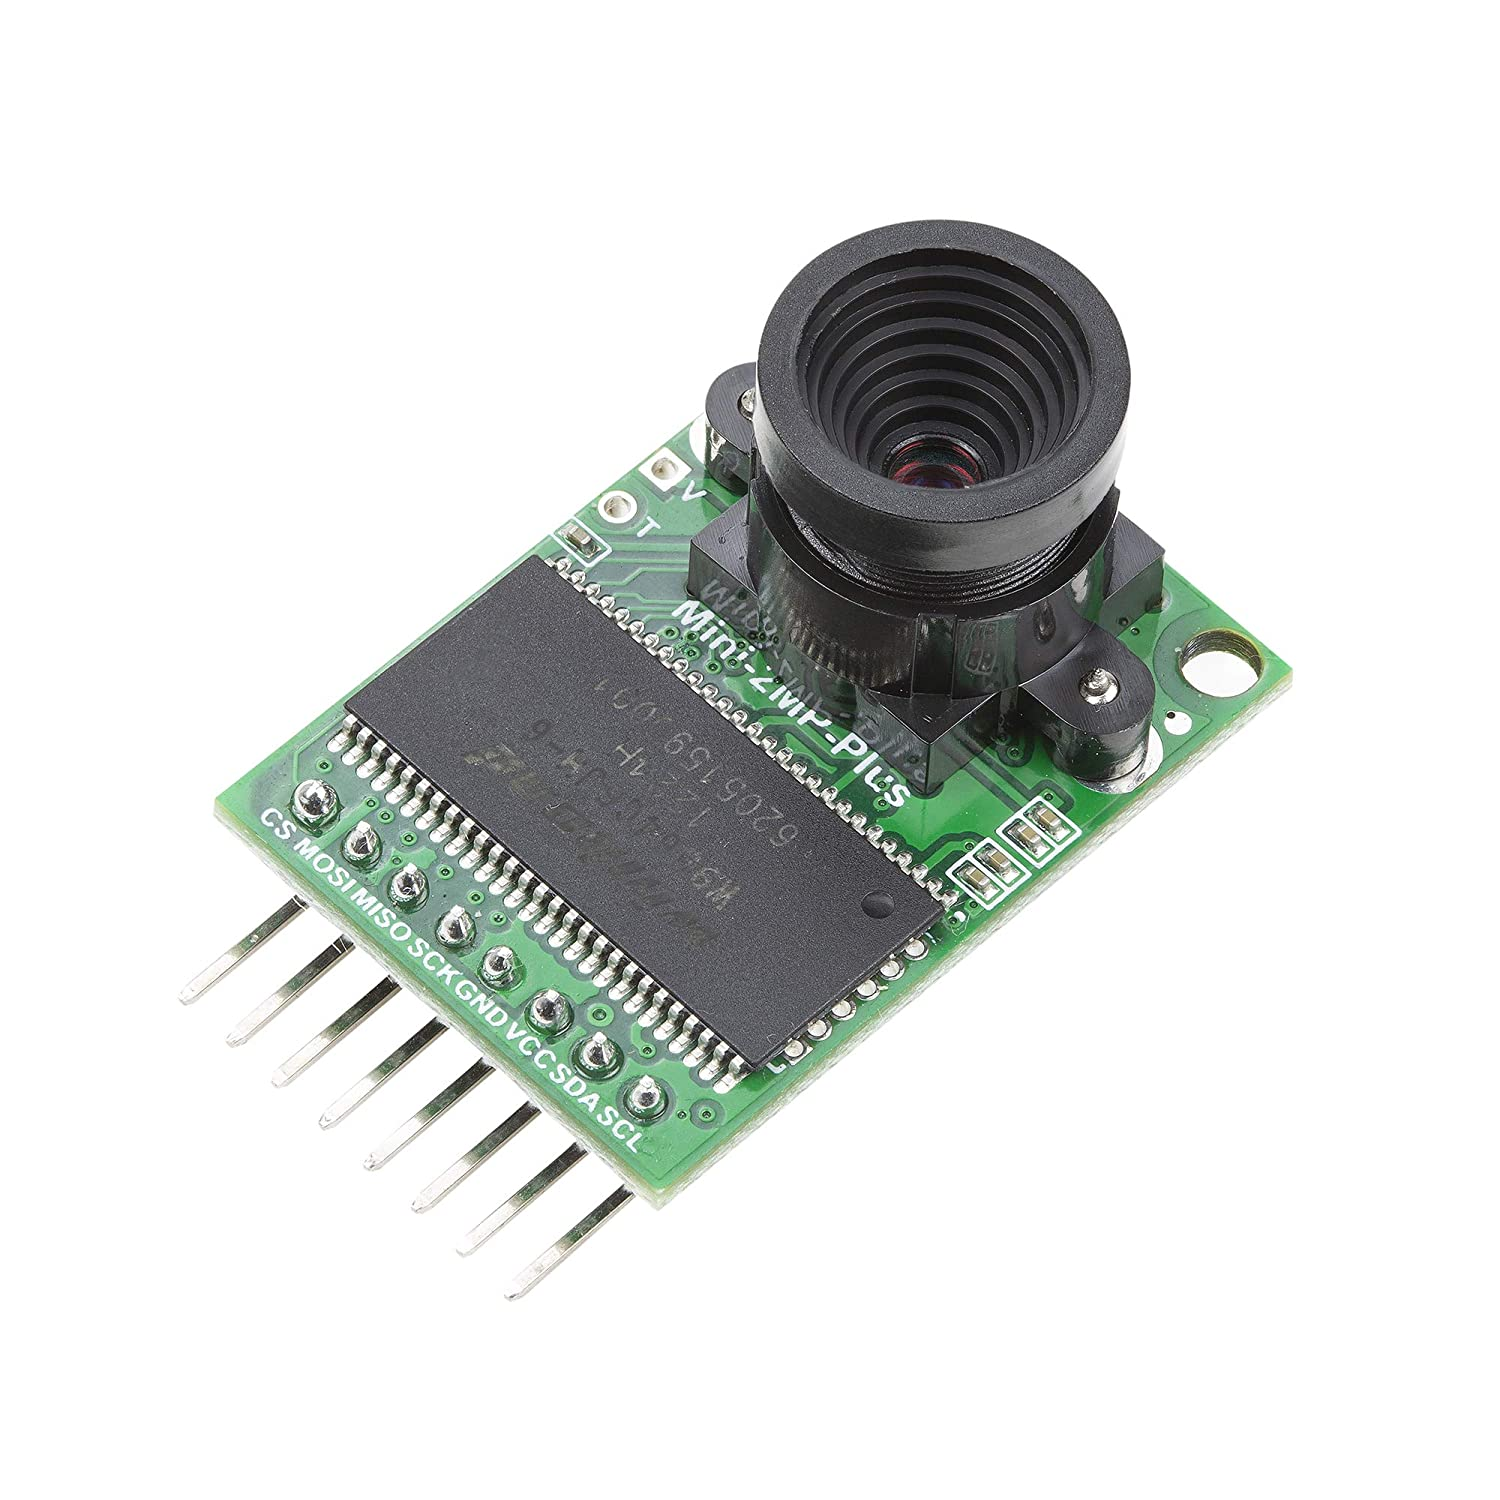
\includegraphics[scale=0.13]{CAM/ov2640/ov2640}
        \quad 
        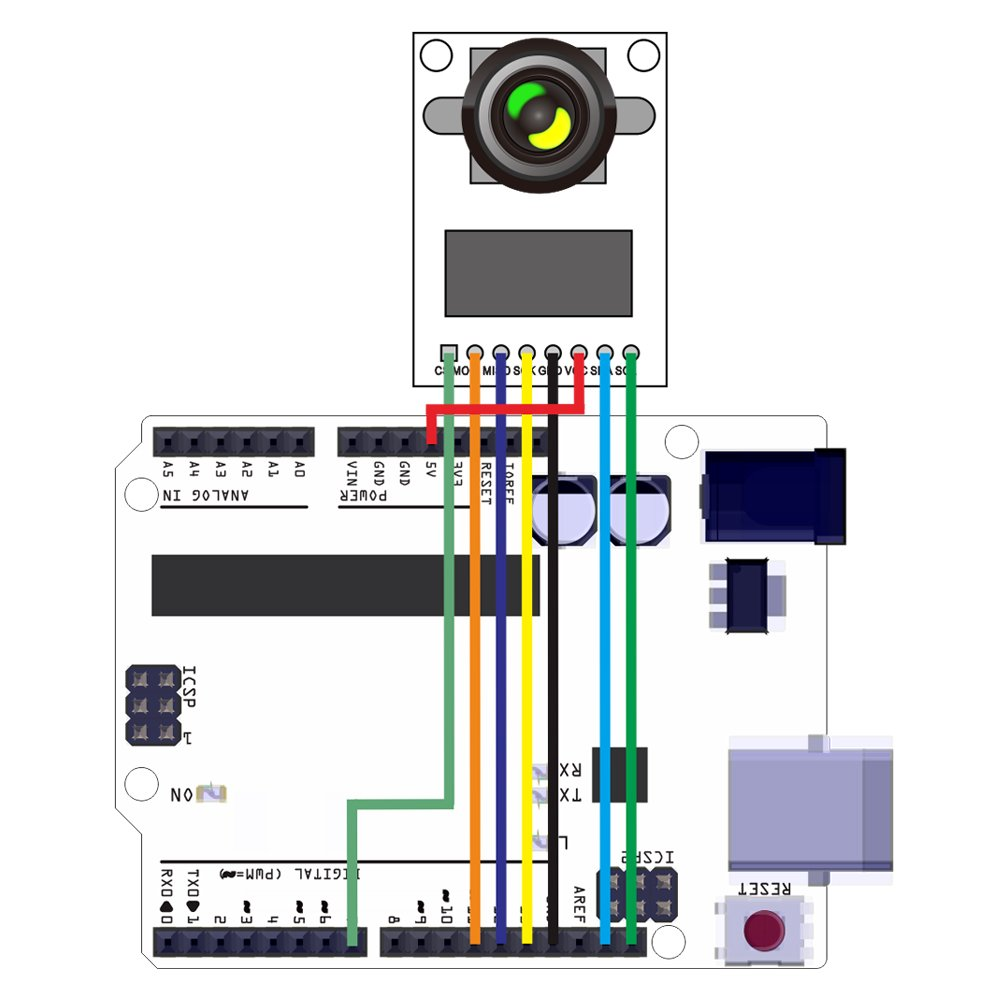
\includegraphics[scale=0.15]{CAM/ov2640/ov2640B4}
        
        \caption{Kamera IMX477 der Firma Arducam; \cite{Arducam:2021}}
    \end{center}    
\end{figure}




\subsection{Pin Configuration of Arducam 0V2640 2MP Mini}

Arducam Mini 2MP OV2640 is a small mini size camera, we can easily embed this camera with any kind of Arduino or other electronics boards, if they have the serial peripheral interface (SPI) and  chip select (CS) . It has has 8 pins, the following figure ~\ref{pin config} shows the functionality of each pin.

\begin{figure}[ht]
    \centering
    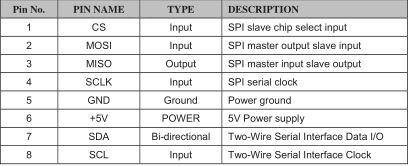
\includegraphics[width=0.8\linewidth]{Nano33BLESense/pin config}
    \caption{ArduCAM Pin Config}
    \label{pin config}
\end{figure}

It offers to add a camera interface with microcontroller the one who dont have camera capability, also there is a option to add multiple cameras with microcontroller.

\section{ArduCAM Interface with Arduino}

ArduCAM OV2640 needs the  SPI and I2C connection with the arduino boards. It will be connecting untill these two connections are make sure. The figure ~\ref{1} shows the ArduCAM connection with Arduino Mega 2560, the same connection will need with the other arduino boards too untill the availabity of  SPI and I2C connection. These ArduCAM cameras are easy to configure with arduino and depends upon the application, it is possible to connect multiple camera with sigle board to make the edge computing application. \href{https://www.arducam.com/product/arducam-2mp-spi-camera-b0067-arduino/}{Arducam Interface}

\begin{figure}[ht]
    \centering
    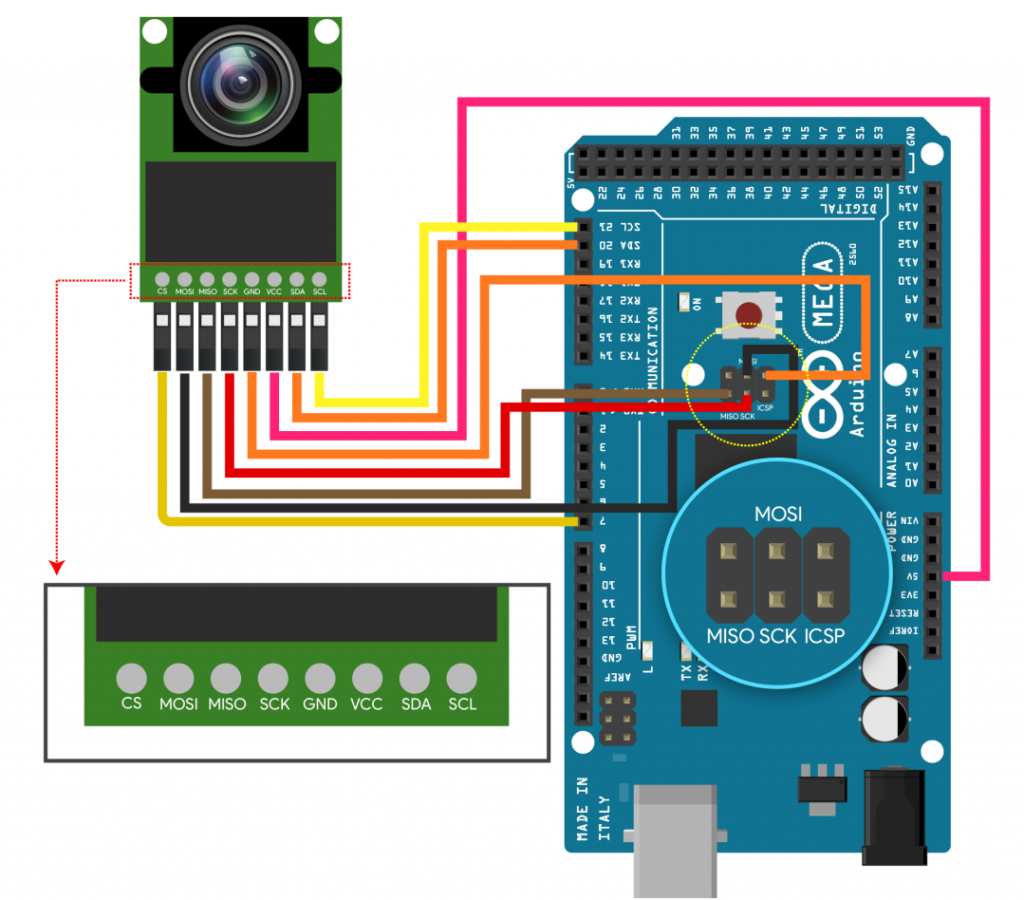
\includegraphics[width=0.6\linewidth]{Nano33BLESense/1}
    \caption{ArduCAM Interface with Arduin Mega 2560} 
    \label{1}
\end{figure}

ArduCAM is very small in size, even it is possible to fix the camera on the Arduino board. There is no external battery require for ArduCam to operate, It needs 5V/70mA operating power supply, so it will get the power from the arduino board too. By having the innovative funcnality with arduino boards, this can be use in the following applications.



\section{ArduCAM Library Introduction}

\url{https://github.com/ArduCAM/Arduino}


Dies ist eine Open-Source-Bibliothek für die Aufnahme von hochauflösenden Standbildern und kurzen Videoclips auf Arduino-basierten Plattformen unter Verwendung der Kameramodule von ArduCAM.
Die Kamera-Breakout-Boards sollten vor dem Anschluss an die Arduino-Boards mit dem ArduCAM-Shield funktionieren.
ArduCAM-Kameramodule der Mini-Serie wie Mini-2MP, Mini-5MP(Plus) können direkt an Arduino-Boards angeschlossen werden.
Zusätzlich zu Arduino kann die Bibliothek auf beliebige Hardware-Plattformen portiert werden, solange sie über eine I2C- und SPI-Schnittstelle verfügen, die auf dieser ArduCAM-Bibliothek basiert.

\bigskip

Now Supported Cameras

\begin{itemize}
  \item OV7660 0.3MP
  \item OV7670 0.3MP
  \item OV7675 0.3MP
  \item OV7725 0.3MP
  \item MT9V111 0.3MP
  \item MT9M112 1.3MP
  \item MT9M001 1.3MP
  \item MT9D111 2MP
  \item OV2640 2MP JPEG
  \item MT9T112 3MP
  \item OV3640 3MP
  \item OV5642 5MP JPEG
  \item OV5640 5MP JPEG
\end{itemize}

Supported MCU Platform

Theoretically support all Arduino families

\begin{itemize}
  \item Arduino UNO R3 (Tested)
  \item Arduino MEGA2560 R3 (Tested)
  \item Arduino Leonardo R3 (Tested)
  \item Arduino Nano (Tested)
  \item Arduino DUE (Tested)
  \item Arduino Genuion 101 (Tested)
  \item Raspberry Pi (Tested)
  \item ESP8266-12 (Tested) (\url{http://www.arducam.com/downloads/ESP8266_UNO/package_ArduCAM_index.json})
  \item Feather M0 (Tested with OV5642)
\end{itemize}


Note: ArduCAM library for ESP8266 is maintained in another repository ESP8266 using a json board manager script.


\section{Libraries Structure}

Die Basisbibliotheken bestehen aus zwei Unterbibliotheken: \FILE{ArduCAM} und \FILE{UTFT4ArduCAM\_SPI}. Diese beiden Bibliotheken sollten direkt unter die Bibliotheken des Arduino-Verzeichnisses kopiert werden, damit sie von der Arduino-IDE erkannt werden.

Die ArduCAM-Bibliothek ist die Kernbibliothek für ArduCAM-Shields. Sie enthält unterstützte Bildsensortreiber und Benutzerland-API-Funktionen, die Befehle zum Erfassen oder Lesen von Bilddaten erteilen. Es gibt auch ein Beispielverzeichnis innerhalb der ArduCAM-Bibliothek, das die meisten Funktionen der ArduCAM-Shields illustriert. Die vorhandenen Beispiele sind Plug-and-Play, ohne dass eine einzige Zeile Code geschrieben werden muss.

Die Bibliothek \FILE{UTFT4ArduCAM\_SPI} ist eine modifizierte Version von UTFT, die von Henning Karlsen geschrieben wurde. Wir haben sie portiert, um das ArduCAM-Shield mit LCD-Bildschirm zu unterstützen. Daher wird die Bibliothek \FILE{UTFT4ArduCAM\_SPI} nur benötigt, wenn das ArduCAM-LF-Modell verwendet wird.




\section{How to use}

Die Bibliotheken sollten vor dem Ausführen von Beispielen konfiguriert werden, andernfalls erhalten Sie eine Fehlermeldung beim Kompilieren.

\subsection{Edit \FILE{memorysaver.h} file}

Öffnen Sie die Datei \FILE{memorysaver.h} im ArduCAM-Ordner und aktivieren Sie die Hardwareplattform und das Kameramodul, das zu Ihrer Hardware passt, indem Sie die Makrodefinition in der Datei auskommentieren oder auskommentieren. Wenn Sie zum Beispiel eine ArduCAM-Mini-2MP haben, sollten Sie die Zeile \PYTHON{\#define OV2640\_MINI\_2MP} auskommentieren und alle anderen Zeilen auskommentieren. Und wenn Sie ein ArduCAM-Shield-V2 und ein OV5642-Kameramodul haben, sollten Sie die Zeile \PYTHON{\#define ARDUCAM\_SHIELD\_V2} und die Zeile \PYTHON{\#define OV5642\_CAM} auskommentieren und dann alle anderen Zeilen.

\subsection{Choose correct CS pin for your camera}

Öffnen Sie eines der Beispiele und verdrahten Sie die SPI- und I2C-Schnittstelle, insbesondere die CS-Pins, entsprechend den Beispielen mit dem ArduCAM-Shield. Hardware und Software sollten konsistent sein, um die Beispiele korrekt auszuführen.

\subsection{Upload the examples}


Im Beispielordner befinden sich sieben Unterverzeichnisse für verschiedene ArduCAM-Modelle und die Host-Anwendung. Der Ordner Mini ist für die Module ArduCAM-Mini-2MP und ArduCAM-Mini-5MP.

\begin{enumerate}
  \item Der Ordner \FILE{Mini\_5MP\_Plus} ist für ArduCAM-Mini-5MP-Plus (OV5640/OV5642) Module.
  \item Der Ordner \FILE{RevC} ist für ArduCAM-Shield-RevC oder ArduCAM-Shield-RevC+ Shields.
  \item Der Ordner \FILE{Shield\_V2} ist für das ArduCAM-Shield-V2 Schild.
  \item Der Ordner \FILE{host\_app} ist die Host-Erfassungs- und Anzeigeanwendung für alle ArduCAM-Module.
  \item Der Ordner \FILE{RaspberryPi} ist eine Beispielanwendung für die Raspberry Pi-Plattform, siehe weitere Anleitung.
  \item Der Ordner \FILE{ESP8266} ist für ArduCAM-ESP8266-UNO-Board-Beispiele für Bibliothekskompatibilität. Bitte versuchen Sie stattdessen, ESP8266 mit dem Skript josn board manager zu repositoryen.
\end{enumerate}


Selecting correct COM port and Arduino boards then upload the sketches.

\bigskip

     
Arducam MINI Kamera Demo Tutorial für Arduino

Arducam Kamera-Schild V2 Demo Tutorial für Arduino

\subsection{How To Connect Bluetooth Module}
Mit dieser Demo

\url{https://github.com/ArduCAM/Arduino/blob/master/ArduCAM/examples/mini/ArduCAM_Mini_Video_Streaming_Bluetooth}

So laden Sie den Host V2:

% \Ausblenden
{

\begin{itemize}
  \item For ArduCAM\_Host\_V2.0\_Mac.app, please refer to this link:
  
         \url{www.arducam.com/downloads/app/ArduCAM_Host_V2.0_Mac.app.zip}
  \item For ArduCAM\_Mini\_V2.0\_Linux\_x86\_64bit, Please refer to this link:
       
       \url{www.arducam.com/downloads/app/ArduCAM_Mini_V2.0_Linux_x86_64bit.zip}
\end{itemize}

}

